% Options for packages loaded elsewhere
\PassOptionsToPackage{unicode}{hyperref}
\PassOptionsToPackage{hyphens}{url}
%
\documentclass[
]{article}
\title{Case Study 2}
\author{Emily Gentles (Writer) \and Weiyi Liu (Coordinator and
Checker) \and Jack McCarthy (Presenter) \and Qinzhe Wang (Coder)}
\date{10/28/2021}

\usepackage{amsmath,amssymb}
\usepackage{lmodern}
\usepackage{iftex}
\ifPDFTeX
  \usepackage[T1]{fontenc}
  \usepackage[utf8]{inputenc}
  \usepackage{textcomp} % provide euro and other symbols
\else % if luatex or xetex
  \usepackage{unicode-math}
  \defaultfontfeatures{Scale=MatchLowercase}
  \defaultfontfeatures[\rmfamily]{Ligatures=TeX,Scale=1}
\fi
% Use upquote if available, for straight quotes in verbatim environments
\IfFileExists{upquote.sty}{\usepackage{upquote}}{}
\IfFileExists{microtype.sty}{% use microtype if available
  \usepackage[]{microtype}
  \UseMicrotypeSet[protrusion]{basicmath} % disable protrusion for tt fonts
}{}
\makeatletter
\@ifundefined{KOMAClassName}{% if non-KOMA class
  \IfFileExists{parskip.sty}{%
    \usepackage{parskip}
  }{% else
    \setlength{\parindent}{0pt}
    \setlength{\parskip}{6pt plus 2pt minus 1pt}}
}{% if KOMA class
  \KOMAoptions{parskip=half}}
\makeatother
\usepackage{xcolor}
\IfFileExists{xurl.sty}{\usepackage{xurl}}{} % add URL line breaks if available
\IfFileExists{bookmark.sty}{\usepackage{bookmark}}{\usepackage{hyperref}}
\hypersetup{
  pdftitle={Case Study 2},
  pdfauthor={Emily Gentles (Writer); Weiyi Liu (Coordinator and Checker); Jack McCarthy (Presenter); Qinzhe Wang (Coder)},
  hidelinks,
  pdfcreator={LaTeX via pandoc}}
\urlstyle{same} % disable monospaced font for URLs
\usepackage[margin=1in]{geometry}
\usepackage{color}
\usepackage{fancyvrb}
\newcommand{\VerbBar}{|}
\newcommand{\VERB}{\Verb[commandchars=\\\{\}]}
\DefineVerbatimEnvironment{Highlighting}{Verbatim}{commandchars=\\\{\}}
% Add ',fontsize=\small' for more characters per line
\usepackage{framed}
\definecolor{shadecolor}{RGB}{248,248,248}
\newenvironment{Shaded}{\begin{snugshade}}{\end{snugshade}}
\newcommand{\AlertTok}[1]{\textcolor[rgb]{0.94,0.16,0.16}{#1}}
\newcommand{\AnnotationTok}[1]{\textcolor[rgb]{0.56,0.35,0.01}{\textbf{\textit{#1}}}}
\newcommand{\AttributeTok}[1]{\textcolor[rgb]{0.77,0.63,0.00}{#1}}
\newcommand{\BaseNTok}[1]{\textcolor[rgb]{0.00,0.00,0.81}{#1}}
\newcommand{\BuiltInTok}[1]{#1}
\newcommand{\CharTok}[1]{\textcolor[rgb]{0.31,0.60,0.02}{#1}}
\newcommand{\CommentTok}[1]{\textcolor[rgb]{0.56,0.35,0.01}{\textit{#1}}}
\newcommand{\CommentVarTok}[1]{\textcolor[rgb]{0.56,0.35,0.01}{\textbf{\textit{#1}}}}
\newcommand{\ConstantTok}[1]{\textcolor[rgb]{0.00,0.00,0.00}{#1}}
\newcommand{\ControlFlowTok}[1]{\textcolor[rgb]{0.13,0.29,0.53}{\textbf{#1}}}
\newcommand{\DataTypeTok}[1]{\textcolor[rgb]{0.13,0.29,0.53}{#1}}
\newcommand{\DecValTok}[1]{\textcolor[rgb]{0.00,0.00,0.81}{#1}}
\newcommand{\DocumentationTok}[1]{\textcolor[rgb]{0.56,0.35,0.01}{\textbf{\textit{#1}}}}
\newcommand{\ErrorTok}[1]{\textcolor[rgb]{0.64,0.00,0.00}{\textbf{#1}}}
\newcommand{\ExtensionTok}[1]{#1}
\newcommand{\FloatTok}[1]{\textcolor[rgb]{0.00,0.00,0.81}{#1}}
\newcommand{\FunctionTok}[1]{\textcolor[rgb]{0.00,0.00,0.00}{#1}}
\newcommand{\ImportTok}[1]{#1}
\newcommand{\InformationTok}[1]{\textcolor[rgb]{0.56,0.35,0.01}{\textbf{\textit{#1}}}}
\newcommand{\KeywordTok}[1]{\textcolor[rgb]{0.13,0.29,0.53}{\textbf{#1}}}
\newcommand{\NormalTok}[1]{#1}
\newcommand{\OperatorTok}[1]{\textcolor[rgb]{0.81,0.36,0.00}{\textbf{#1}}}
\newcommand{\OtherTok}[1]{\textcolor[rgb]{0.56,0.35,0.01}{#1}}
\newcommand{\PreprocessorTok}[1]{\textcolor[rgb]{0.56,0.35,0.01}{\textit{#1}}}
\newcommand{\RegionMarkerTok}[1]{#1}
\newcommand{\SpecialCharTok}[1]{\textcolor[rgb]{0.00,0.00,0.00}{#1}}
\newcommand{\SpecialStringTok}[1]{\textcolor[rgb]{0.31,0.60,0.02}{#1}}
\newcommand{\StringTok}[1]{\textcolor[rgb]{0.31,0.60,0.02}{#1}}
\newcommand{\VariableTok}[1]{\textcolor[rgb]{0.00,0.00,0.00}{#1}}
\newcommand{\VerbatimStringTok}[1]{\textcolor[rgb]{0.31,0.60,0.02}{#1}}
\newcommand{\WarningTok}[1]{\textcolor[rgb]{0.56,0.35,0.01}{\textbf{\textit{#1}}}}
\usepackage{graphicx}
\makeatletter
\def\maxwidth{\ifdim\Gin@nat@width>\linewidth\linewidth\else\Gin@nat@width\fi}
\def\maxheight{\ifdim\Gin@nat@height>\textheight\textheight\else\Gin@nat@height\fi}
\makeatother
% Scale images if necessary, so that they will not overflow the page
% margins by default, and it is still possible to overwrite the defaults
% using explicit options in \includegraphics[width, height, ...]{}
\setkeys{Gin}{width=\maxwidth,height=\maxheight,keepaspectratio}
% Set default figure placement to htbp
\makeatletter
\def\fps@figure{htbp}
\makeatother
\setlength{\emergencystretch}{3em} % prevent overfull lines
\providecommand{\tightlist}{%
  \setlength{\itemsep}{0pt}\setlength{\parskip}{0pt}}
\setcounter{secnumdepth}{-\maxdimen} % remove section numbering
\usepackage{booktabs}
\usepackage{longtable}
\usepackage{array}
\usepackage{multirow}
\usepackage{wrapfig}
\usepackage{float}
\usepackage{colortbl}
\usepackage{pdflscape}
\usepackage{tabu}
\usepackage{threeparttable}
\usepackage{threeparttablex}
\usepackage[normalem]{ulem}
\usepackage{makecell}
\usepackage{xcolor}
\ifLuaTeX
  \usepackage{selnolig}  % disable illegal ligatures
\fi

\begin{document}
\maketitle

Tools -\textgreater{} Global Options -\textgreater{} Code
-\textgreater{} Display -\textgreater{} Show Margin

\begin{Shaded}
\begin{Highlighting}[]
\CommentTok{\# contains info about the aggregate counts of voters who actually voted by demographic variables}

\NormalTok{votes }\OtherTok{\textless{}{-}} \FunctionTok{read.table}\NormalTok{(}\StringTok{"history\_stats\_20201103.txt"}\NormalTok{, }\AttributeTok{header =} \ConstantTok{TRUE}\NormalTok{, }\AttributeTok{fill =} \ConstantTok{TRUE}\NormalTok{, }\AttributeTok{sep =} \StringTok{\textquotesingle{}}\SpecialCharTok{\textbackslash{}t}\StringTok{\textquotesingle{}}\NormalTok{)}

\CommentTok{\# contains info about the aggregate counts of registered voters by demographic variables}
\NormalTok{registers }\OtherTok{\textless{}{-}} \FunctionTok{read.table}\NormalTok{(}\StringTok{"voter\_stats\_20201103.txt"}\NormalTok{, }\AttributeTok{header =} \ConstantTok{TRUE}\NormalTok{, }\AttributeTok{fill =} \ConstantTok{TRUE}\NormalTok{, }\AttributeTok{sep =} \StringTok{\textquotesingle{}}\SpecialCharTok{\textbackslash{}t}\StringTok{\textquotesingle{}}\NormalTok{)}
\end{Highlighting}
\end{Shaded}

\begin{Shaded}
\begin{Highlighting}[]
\CommentTok{\# set "" or " " to NA}
\NormalTok{registers[registers }\SpecialCharTok{\%in\%} \FunctionTok{c}\NormalTok{(}\StringTok{""}\NormalTok{, }\StringTok{" "}\NormalTok{)] }\OtherTok{\textless{}{-}} \ConstantTok{NA}
\NormalTok{votes[votes }\SpecialCharTok{==} \StringTok{" "}\NormalTok{] }\OtherTok{\textless{}{-}} \ConstantTok{NA}

\CommentTok{\# unique(registers$election\_date) \# "11/03/2020" NA }
\CommentTok{\# unique(registers$stats\_type) \# "history" NA  }
\CommentTok{\# unique(registers$update\_date) \# "01/13/2021" NA     }

\CommentTok{\# remove above three columns}

\NormalTok{registers }\OtherTok{\textless{}{-}}\NormalTok{ registers }\SpecialCharTok{\%\textgreater{}\%}
  \FunctionTok{select}\NormalTok{(}\SpecialCharTok{{-}}\FunctionTok{c}\NormalTok{(election\_date, stats\_type, update\_date)) }\SpecialCharTok{\%\textgreater{}\%}
  \FunctionTok{mutate}\NormalTok{(}\AttributeTok{total\_voters2 =} \FunctionTok{as.numeric}\NormalTok{(total\_voters))}

\NormalTok{votes }\OtherTok{\textless{}{-}}\NormalTok{ votes }\SpecialCharTok{\%\textgreater{}\%}
  \FunctionTok{select}\NormalTok{(}\SpecialCharTok{{-}}\FunctionTok{c}\NormalTok{(election\_date, stats\_type, update\_date)) }\SpecialCharTok{\%\textgreater{}\%}
  \FunctionTok{mutate}\NormalTok{(}\AttributeTok{total\_voters =} \FunctionTok{as.numeric}\NormalTok{(total\_voters))}
\end{Highlighting}
\end{Shaded}

\begin{Shaded}
\begin{Highlighting}[]
\CommentTok{\# aggregated\_data \textless{}{-} aggregate(voter$total\_voters,}
\CommentTok{\#                              list(county\_desc = voter$county\_desc,}
\CommentTok{\#                                   age=voter$age,}
\CommentTok{\#                                   party\_cd=voter$party\_cd, }
\CommentTok{\#                                   race\_code = voter$race\_code, }
\CommentTok{\#                                   sex\_code = voter$sex\_code, }
\CommentTok{\#                                   precinct\_abbrv = voter$precinct\_abbrv,}
\CommentTok{\#                                   ethnic\_code = voter$ethnic\_code,}
\CommentTok{\#                                   voting\_method\_desc = voter$voting\_method\_desc),}
\CommentTok{\#                              sum)}
\CommentTok{\# }
\CommentTok{\# aggregated\_data \textless{}{-} aggregated\_data \%\textgreater{}\%}
\CommentTok{\#   rename(total\_voters = x)}
\end{Highlighting}
\end{Shaded}

\begin{Shaded}
\begin{Highlighting}[]
\NormalTok{votes }\OtherTok{\textless{}{-}}\NormalTok{ votes }\SpecialCharTok{\%\textgreater{}\%}
  \FunctionTok{group\_by}\NormalTok{(county\_desc, age, party\_cd, race\_code, ethnic\_code, sex\_code) }\SpecialCharTok{\%\textgreater{}\%}
  \FunctionTok{summarize}\NormalTok{(}\AttributeTok{total\_vot =} \FunctionTok{sum}\NormalTok{(total\_voters, }\AttributeTok{na.rm =}\NormalTok{ T))}
\end{Highlighting}
\end{Shaded}

\begin{verbatim}
## `summarise()` has grouped output by 'county_desc', 'age', 'party_cd', 'race_code', 'ethnic_code'. You can override using the `.groups` argument.
\end{verbatim}

\begin{Shaded}
\begin{Highlighting}[]
\NormalTok{data }\OtherTok{\textless{}{-}}\NormalTok{ registers }\SpecialCharTok{\%\textgreater{}\%}
  \FunctionTok{group\_by}\NormalTok{(county\_desc, party\_cd, race\_code, ethnic\_code, sex\_code, age) }\SpecialCharTok{\%\textgreater{}\%}
  \FunctionTok{summarize}\NormalTok{(}\AttributeTok{total\_reg =} \FunctionTok{sum}\NormalTok{(total\_voters2, }\AttributeTok{na.rm =}\NormalTok{ T)) }\SpecialCharTok{\%\textgreater{}\%}
  \FunctionTok{left\_join}\NormalTok{(votes, }\AttributeTok{by =} \FunctionTok{c}\NormalTok{(}
    \StringTok{"county\_desc"}\NormalTok{, }\StringTok{"age"}\NormalTok{, }\StringTok{"party\_cd"}\NormalTok{, }\StringTok{"race\_code"}\NormalTok{, }\StringTok{"ethnic\_code"}\NormalTok{, }\StringTok{"sex\_code"}
\NormalTok{  ))}
\end{Highlighting}
\end{Shaded}

\begin{verbatim}
## `summarise()` has grouped output by 'county_desc', 'party_cd', 'race_code', 'ethnic_code', 'sex_code'. You can override using the `.groups` argument.
\end{verbatim}

\begin{Shaded}
\begin{Highlighting}[]
\NormalTok{data }\OtherTok{\textless{}{-}}\NormalTok{ data }\SpecialCharTok{\%\textgreater{}\%}
  \FunctionTok{mutate}\NormalTok{(}
    \AttributeTok{total\_vot =} \FunctionTok{as.numeric}\NormalTok{(total\_vot), }
    \AttributeTok{total\_reg =} \FunctionTok{as.numeric}\NormalTok{(total\_reg), }
    \AttributeTok{county\_desc =} \FunctionTok{as.factor}\NormalTok{(county\_desc), }
    \AttributeTok{party\_cd =} \FunctionTok{as.factor}\NormalTok{(party\_cd), }
    \AttributeTok{race\_code =} \FunctionTok{as.factor}\NormalTok{(race\_code), }
    \AttributeTok{sex\_code =} \FunctionTok{as.factor}\NormalTok{(sex\_code), }
    \AttributeTok{ethnic\_code =} \FunctionTok{as.factor}\NormalTok{(ethnic\_code), }
    \AttributeTok{age =} \FunctionTok{as.factor}\NormalTok{(age)}
\NormalTok{  )}
\end{Highlighting}
\end{Shaded}

\begin{Shaded}
\begin{Highlighting}[]
\CommentTok{\# 13066 rows}
\NormalTok{data }\OtherTok{\textless{}{-}}\NormalTok{ data }\SpecialCharTok{\%\textgreater{}\%}
  \FunctionTok{filter}\NormalTok{(}\SpecialCharTok{!}\FunctionTok{is.na}\NormalTok{(total\_reg)) }\SpecialCharTok{\%\textgreater{}\%}
  \FunctionTok{mutate}\NormalTok{(}
    \AttributeTok{total\_vot =} \FunctionTok{case\_when}\NormalTok{(}
      \FunctionTok{is.na}\NormalTok{(total\_vot) }\SpecialCharTok{\textasciitilde{}} \DecValTok{0}\NormalTok{,}
\NormalTok{      total\_vot }\SpecialCharTok{\textgreater{}}\NormalTok{ total\_reg }\SpecialCharTok{\textasciitilde{}}\NormalTok{ total\_reg,}
      \ConstantTok{TRUE} \SpecialCharTok{\textasciitilde{}}\NormalTok{ total\_vot}
\NormalTok{    )}
\NormalTok{  ) }\SpecialCharTok{\%\textgreater{}\%}
  \FunctionTok{drop\_na}\NormalTok{()}
\end{Highlighting}
\end{Shaded}

\begin{Shaded}
\begin{Highlighting}[]
\FunctionTok{set.seed}\NormalTok{(}\DecValTok{1031}\NormalTok{)}

\NormalTok{counties }\OtherTok{\textless{}{-}} \FunctionTok{sample}\NormalTok{(}\FunctionTok{unique}\NormalTok{(data}\SpecialCharTok{$}\NormalTok{county\_desc), }\DecValTok{30}\NormalTok{)}

\NormalTok{data }\OtherTok{\textless{}{-}}\NormalTok{ data }\SpecialCharTok{\%\textgreater{}\%}
  \FunctionTok{filter}\NormalTok{(county\_desc }\SpecialCharTok{\%in\%}\NormalTok{ counties)}
\end{Highlighting}
\end{Shaded}

\hypertarget{eda}{%
\section{EDA}\label{eda}}

\begin{Shaded}
\begin{Highlighting}[]
\NormalTok{turnout\_rate }\OtherTok{\textless{}{-}} \FunctionTok{sum}\NormalTok{(data}\SpecialCharTok{$}\NormalTok{total\_vot) }\SpecialCharTok{/} \FunctionTok{sum}\NormalTok{(data}\SpecialCharTok{$}\NormalTok{total\_reg)}

\FunctionTok{data.frame}\NormalTok{(}\AttributeTok{group =} \StringTok{"Total"}\NormalTok{, }\AttributeTok{turnout\_rate =}\NormalTok{ turnout\_rate)}
\end{Highlighting}
\end{Shaded}

\begin{verbatim}
##   group turnout_rate
## 1 Total    0.6533629
\end{verbatim}

\hypertarget{turnout-rate}{%
\subsubsection{turnout rate}\label{turnout-rate}}

\begin{Shaded}
\begin{Highlighting}[]
\NormalTok{data }\SpecialCharTok{\%\textgreater{}\%}
  \FunctionTok{group\_by}\NormalTok{(county\_desc) }\SpecialCharTok{\%\textgreater{}\%}
  \FunctionTok{summarise}\NormalTok{(}\AttributeTok{total\_reg =} \FunctionTok{sum}\NormalTok{(total\_reg),}
            \AttributeTok{total\_vot =} \FunctionTok{sum}\NormalTok{(total\_vot), }\AttributeTok{.groups =} \StringTok{"drop"}\NormalTok{) }\SpecialCharTok{\%\textgreater{}\%}
  \FunctionTok{mutate}\NormalTok{(}\AttributeTok{turnout\_rate =}\NormalTok{ total\_vot }\SpecialCharTok{/}\NormalTok{ total\_reg) }\SpecialCharTok{\%\textgreater{}\%}
  \FunctionTok{ggplot}\NormalTok{( }\FunctionTok{aes}\NormalTok{(}\AttributeTok{x =}\NormalTok{ county\_desc, }\AttributeTok{y =}\NormalTok{ turnout\_rate)) }\SpecialCharTok{+}
    \FunctionTok{geom\_bar}\NormalTok{(}\AttributeTok{stat =} \StringTok{"identity"}\NormalTok{) }\SpecialCharTok{+}
    \FunctionTok{ylim}\NormalTok{(}\DecValTok{0}\NormalTok{,}\DecValTok{1}\NormalTok{) }\SpecialCharTok{+}
    \FunctionTok{xlab}\NormalTok{(}\StringTok{"County"}\NormalTok{) }\SpecialCharTok{+} \FunctionTok{ylab}\NormalTok{(}\StringTok{"Turnout rate"}\NormalTok{) }\SpecialCharTok{+}
    \FunctionTok{geom\_text}\NormalTok{(}\FunctionTok{aes}\NormalTok{(}\AttributeTok{label=}\FunctionTok{format}\NormalTok{(turnout\_rate, }\AttributeTok{digits =} \DecValTok{2}\NormalTok{)), }\AttributeTok{hjust =} \SpecialCharTok{{-}}\FloatTok{0.3}\NormalTok{) }\SpecialCharTok{+}
    \FunctionTok{ggtitle}\NormalTok{(}\StringTok{"Turnout rate vs. County"}\NormalTok{) }\SpecialCharTok{+}
      \FunctionTok{theme}\NormalTok{(}\AttributeTok{plot.title =} \FunctionTok{element\_text}\NormalTok{(}\AttributeTok{hjust =} \FloatTok{0.5}\NormalTok{)) }\SpecialCharTok{+}
    \FunctionTok{coord\_flip}\NormalTok{()}
\end{Highlighting}
\end{Shaded}

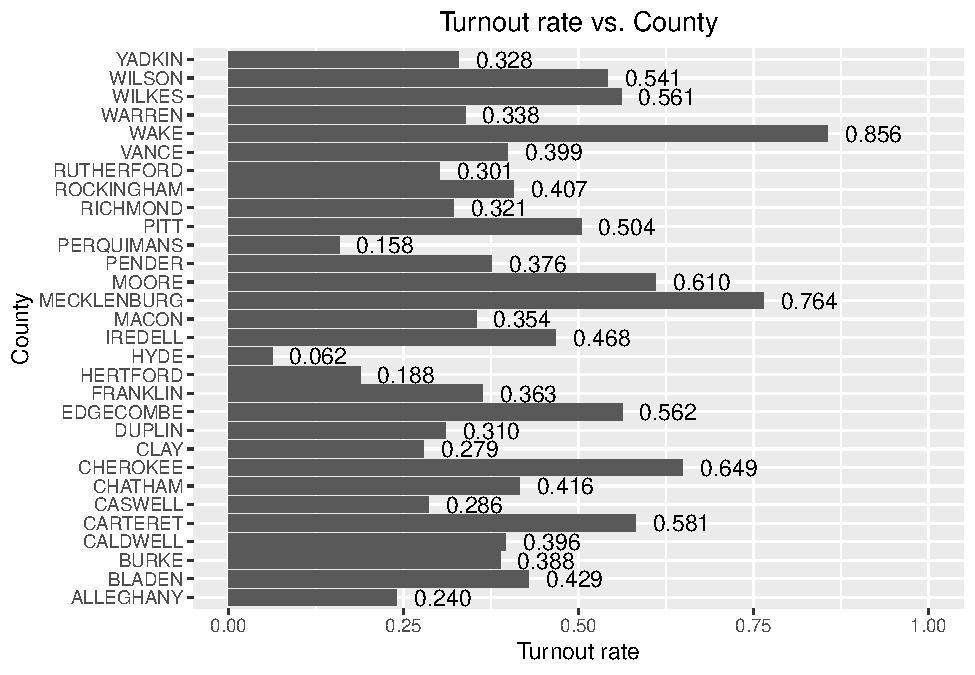
\includegraphics{CS2_files/figure-latex/unnamed-chunk-8-1.pdf}

\hypertarget{race}{%
\subsubsection{race}\label{race}}

\begin{Shaded}
\begin{Highlighting}[]
\NormalTok{data }\SpecialCharTok{\%\textgreater{}\%}
  \FunctionTok{group\_by}\NormalTok{(race\_code) }\SpecialCharTok{\%\textgreater{}\%}
  \FunctionTok{summarise}\NormalTok{(}\AttributeTok{total\_reg =} \FunctionTok{sum}\NormalTok{(total\_reg),}
            \AttributeTok{total\_vot =} \FunctionTok{sum}\NormalTok{(total\_vot), }\AttributeTok{.groups =} \StringTok{"drop"}\NormalTok{) }\SpecialCharTok{\%\textgreater{}\%}
  \FunctionTok{mutate}\NormalTok{(}\AttributeTok{turnout\_rate =}\NormalTok{ total\_vot }\SpecialCharTok{/}\NormalTok{ total\_reg) }\SpecialCharTok{\%\textgreater{}\%}
  \FunctionTok{select}\NormalTok{(}\AttributeTok{group =}\NormalTok{ race\_code, turnout\_rate) }\SpecialCharTok{\%\textgreater{}\%}
  \FunctionTok{ggplot}\NormalTok{( }\FunctionTok{aes}\NormalTok{(}\AttributeTok{x =}\NormalTok{ group, }\AttributeTok{y =}\NormalTok{ turnout\_rate)) }\SpecialCharTok{+}
  \FunctionTok{geom\_bar}\NormalTok{(}\AttributeTok{stat =} \StringTok{"identity"}\NormalTok{) }\SpecialCharTok{+}
  \FunctionTok{ylim}\NormalTok{(}\DecValTok{0}\NormalTok{,}\DecValTok{1}\NormalTok{) }\SpecialCharTok{+}
  \FunctionTok{xlab}\NormalTok{(}\StringTok{"Race"}\NormalTok{) }\SpecialCharTok{+} \FunctionTok{ylab}\NormalTok{(}\StringTok{"Turnout rate"}\NormalTok{) }\SpecialCharTok{+}
  \FunctionTok{geom\_text}\NormalTok{(}\FunctionTok{aes}\NormalTok{(}\AttributeTok{label=}\FunctionTok{format}\NormalTok{(turnout\_rate, }\AttributeTok{digits =} \DecValTok{2}\NormalTok{)), }\AttributeTok{vjust =} \SpecialCharTok{{-}}\FloatTok{0.5}\NormalTok{) }\SpecialCharTok{+}
  \FunctionTok{ggtitle}\NormalTok{(}\StringTok{"Turnout rate vs. Race"}\NormalTok{) }\SpecialCharTok{+}
    \FunctionTok{theme}\NormalTok{(}\AttributeTok{plot.title =} \FunctionTok{element\_text}\NormalTok{(}\AttributeTok{hjust =} \FloatTok{0.5}\NormalTok{))}
\end{Highlighting}
\end{Shaded}

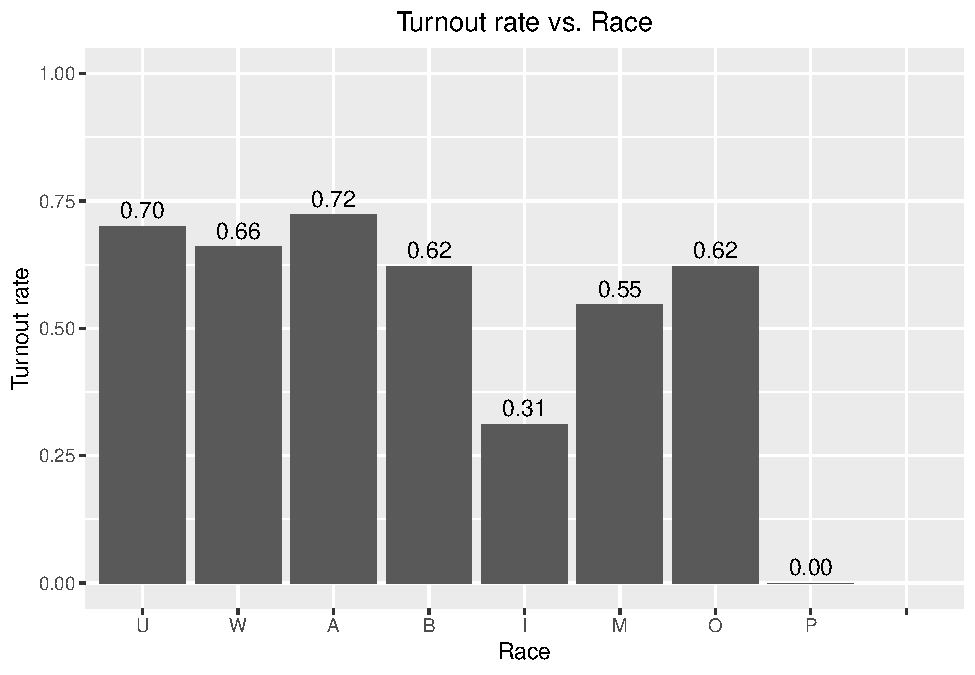
\includegraphics{CS2_files/figure-latex/unnamed-chunk-9-1.pdf}

\hypertarget{party}{%
\subsubsection{party}\label{party}}

\begin{Shaded}
\begin{Highlighting}[]
\NormalTok{data }\SpecialCharTok{\%\textgreater{}\%}
  \FunctionTok{group\_by}\NormalTok{(party\_cd) }\SpecialCharTok{\%\textgreater{}\%}
  \FunctionTok{summarise}\NormalTok{(}\AttributeTok{total\_reg =} \FunctionTok{sum}\NormalTok{(total\_reg),}
            \AttributeTok{total\_vot =} \FunctionTok{sum}\NormalTok{(total\_vot), }\AttributeTok{.groups =} \StringTok{"drop"}\NormalTok{) }\SpecialCharTok{\%\textgreater{}\%}
  \FunctionTok{mutate}\NormalTok{(}\AttributeTok{turnout\_rate =}\NormalTok{ total\_vot }\SpecialCharTok{/}\NormalTok{ total\_reg) }\SpecialCharTok{\%\textgreater{}\%}
  \FunctionTok{select}\NormalTok{(}\AttributeTok{group =}\NormalTok{ party\_cd, turnout\_rate) }\SpecialCharTok{\%\textgreater{}\%}
  \FunctionTok{ggplot}\NormalTok{( }\FunctionTok{aes}\NormalTok{(}\AttributeTok{x =}\NormalTok{ group, }\AttributeTok{y =}\NormalTok{ turnout\_rate)) }\SpecialCharTok{+}
  \FunctionTok{geom\_bar}\NormalTok{(}\AttributeTok{stat =} \StringTok{"identity"}\NormalTok{) }\SpecialCharTok{+}
  \FunctionTok{ylim}\NormalTok{(}\DecValTok{0}\NormalTok{,}\DecValTok{1}\NormalTok{) }\SpecialCharTok{+}
  \FunctionTok{xlab}\NormalTok{(}\StringTok{"Party"}\NormalTok{) }\SpecialCharTok{+} \FunctionTok{ylab}\NormalTok{(}\StringTok{"Turnout rate"}\NormalTok{) }\SpecialCharTok{+}
  \FunctionTok{geom\_text}\NormalTok{(}\FunctionTok{aes}\NormalTok{(}\AttributeTok{label=}\FunctionTok{format}\NormalTok{(turnout\_rate, }\AttributeTok{digits =} \DecValTok{2}\NormalTok{)), }\AttributeTok{vjust =} \SpecialCharTok{{-}}\FloatTok{0.5}\NormalTok{) }\SpecialCharTok{+}
  \FunctionTok{ggtitle}\NormalTok{(}\StringTok{"Turnout rate vs. Party"}\NormalTok{) }\SpecialCharTok{+}
    \FunctionTok{theme}\NormalTok{(}\AttributeTok{plot.title =} \FunctionTok{element\_text}\NormalTok{(}\AttributeTok{hjust =} \FloatTok{0.5}\NormalTok{))}
\end{Highlighting}
\end{Shaded}

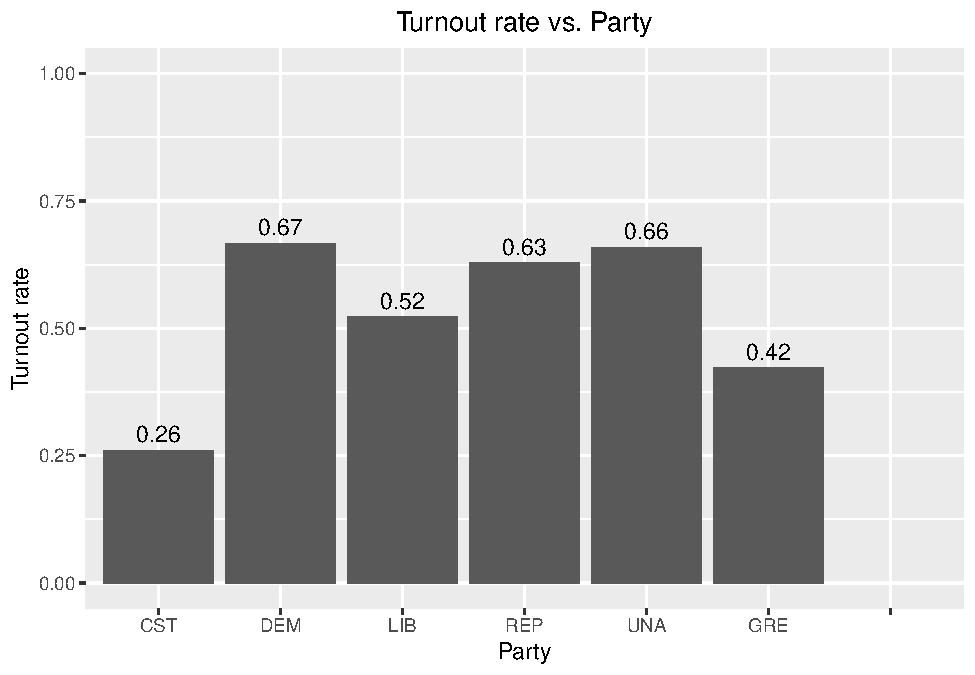
\includegraphics{CS2_files/figure-latex/unnamed-chunk-10-1.pdf}

\hypertarget{ethnic-groups}{%
\subsubsection{ethnic groups}\label{ethnic-groups}}

\begin{Shaded}
\begin{Highlighting}[]
\NormalTok{data }\SpecialCharTok{\%\textgreater{}\%}
  \FunctionTok{group\_by}\NormalTok{(ethnic\_code) }\SpecialCharTok{\%\textgreater{}\%}
  \FunctionTok{summarise}\NormalTok{(}\AttributeTok{total\_reg =} \FunctionTok{sum}\NormalTok{(total\_reg),}
            \AttributeTok{total\_vot =} \FunctionTok{sum}\NormalTok{(total\_vot), }\AttributeTok{.groups =} \StringTok{"drop"}\NormalTok{) }\SpecialCharTok{\%\textgreater{}\%}
  \FunctionTok{mutate}\NormalTok{(}\AttributeTok{turnout\_rate =}\NormalTok{ total\_vot }\SpecialCharTok{/}\NormalTok{ total\_reg) }\SpecialCharTok{\%\textgreater{}\%}
  \FunctionTok{select}\NormalTok{(}\AttributeTok{group =}\NormalTok{ ethnic\_code, turnout\_rate) }\SpecialCharTok{\%\textgreater{}\%}
  \FunctionTok{ggplot}\NormalTok{( }\FunctionTok{aes}\NormalTok{(}\AttributeTok{x =}\NormalTok{ group, }\AttributeTok{y =}\NormalTok{ turnout\_rate)) }\SpecialCharTok{+}
  \FunctionTok{geom\_bar}\NormalTok{(}\AttributeTok{stat =} \StringTok{"identity"}\NormalTok{) }\SpecialCharTok{+}
  \FunctionTok{ylim}\NormalTok{(}\DecValTok{0}\NormalTok{,}\DecValTok{1}\NormalTok{) }\SpecialCharTok{+}
  \FunctionTok{xlab}\NormalTok{(}\StringTok{"Ethnic"}\NormalTok{) }\SpecialCharTok{+} \FunctionTok{ylab}\NormalTok{(}\StringTok{"Turnout rate"}\NormalTok{) }\SpecialCharTok{+}
  \FunctionTok{geom\_text}\NormalTok{(}\FunctionTok{aes}\NormalTok{(}\AttributeTok{label=}\FunctionTok{format}\NormalTok{(turnout\_rate, }\AttributeTok{digits =} \DecValTok{2}\NormalTok{)), }\AttributeTok{vjust =} \SpecialCharTok{{-}}\FloatTok{0.5}\NormalTok{) }\SpecialCharTok{+}
  \FunctionTok{ggtitle}\NormalTok{(}\StringTok{"Turnout rate vs. Ethnic"}\NormalTok{) }\SpecialCharTok{+}
    \FunctionTok{theme}\NormalTok{(}\AttributeTok{plot.title =} \FunctionTok{element\_text}\NormalTok{(}\AttributeTok{hjust =} \FloatTok{0.5}\NormalTok{))}
\end{Highlighting}
\end{Shaded}

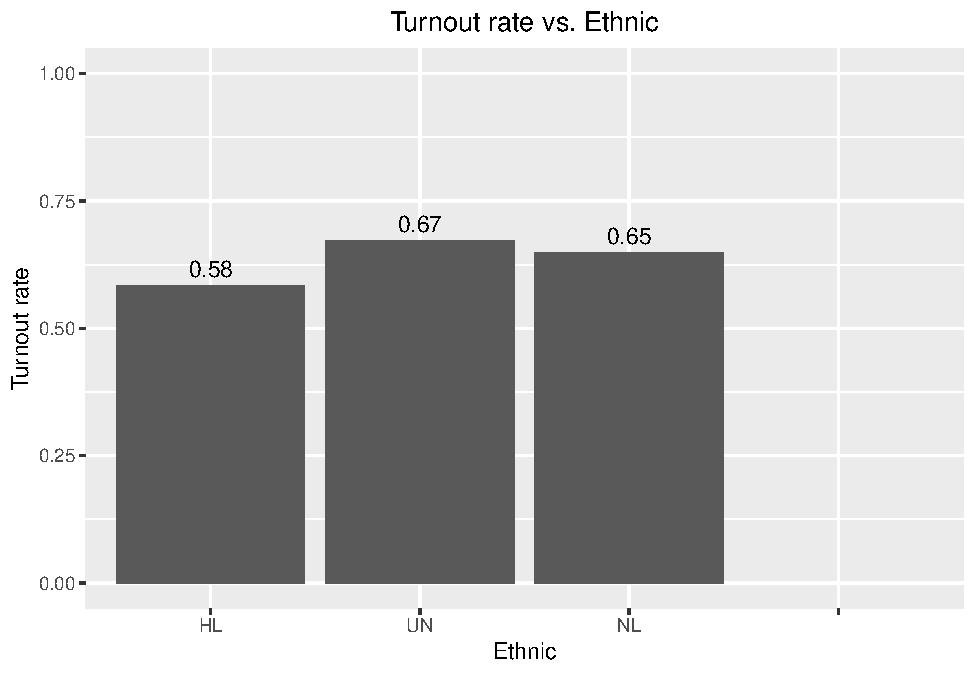
\includegraphics{CS2_files/figure-latex/unnamed-chunk-11-1.pdf}

\hypertarget{sex}{%
\subsubsection{Sex}\label{sex}}

\begin{Shaded}
\begin{Highlighting}[]
\NormalTok{data }\SpecialCharTok{\%\textgreater{}\%}
  \FunctionTok{group\_by}\NormalTok{(sex\_code) }\SpecialCharTok{\%\textgreater{}\%}
  \FunctionTok{summarise}\NormalTok{(}\AttributeTok{total\_reg =} \FunctionTok{sum}\NormalTok{(total\_reg),}
            \AttributeTok{total\_vot =} \FunctionTok{sum}\NormalTok{(total\_vot), }\AttributeTok{.groups =} \StringTok{"drop"}\NormalTok{) }\SpecialCharTok{\%\textgreater{}\%}
  \FunctionTok{mutate}\NormalTok{(}\AttributeTok{turnout\_rate =}\NormalTok{ total\_vot }\SpecialCharTok{/}\NormalTok{ total\_reg) }\SpecialCharTok{\%\textgreater{}\%}
  \FunctionTok{select}\NormalTok{(}\AttributeTok{group =}\NormalTok{ sex\_code, turnout\_rate) }\SpecialCharTok{\%\textgreater{}\%}
  \FunctionTok{ggplot}\NormalTok{( }\FunctionTok{aes}\NormalTok{(}\AttributeTok{x =}\NormalTok{ group, }\AttributeTok{y =}\NormalTok{ turnout\_rate)) }\SpecialCharTok{+}
  \FunctionTok{geom\_bar}\NormalTok{(}\AttributeTok{stat =} \StringTok{"identity"}\NormalTok{) }\SpecialCharTok{+}
  \FunctionTok{ylim}\NormalTok{(}\DecValTok{0}\NormalTok{,}\DecValTok{1}\NormalTok{) }\SpecialCharTok{+}
  \FunctionTok{xlab}\NormalTok{(}\StringTok{"Sex"}\NormalTok{) }\SpecialCharTok{+} \FunctionTok{ylab}\NormalTok{(}\StringTok{"Turnout rate"}\NormalTok{) }\SpecialCharTok{+}
  \FunctionTok{geom\_text}\NormalTok{(}\FunctionTok{aes}\NormalTok{(}\AttributeTok{label=}\FunctionTok{format}\NormalTok{(turnout\_rate, }\AttributeTok{digits =} \DecValTok{2}\NormalTok{)), }\AttributeTok{vjust =} \SpecialCharTok{{-}}\FloatTok{0.5}\NormalTok{) }\SpecialCharTok{+}
  \FunctionTok{ggtitle}\NormalTok{(}\StringTok{"Turnout rate vs. Sex"}\NormalTok{) }\SpecialCharTok{+}
    \FunctionTok{theme}\NormalTok{(}\AttributeTok{plot.title =} \FunctionTok{element\_text}\NormalTok{(}\AttributeTok{hjust =} \FloatTok{0.5}\NormalTok{))}
\end{Highlighting}
\end{Shaded}

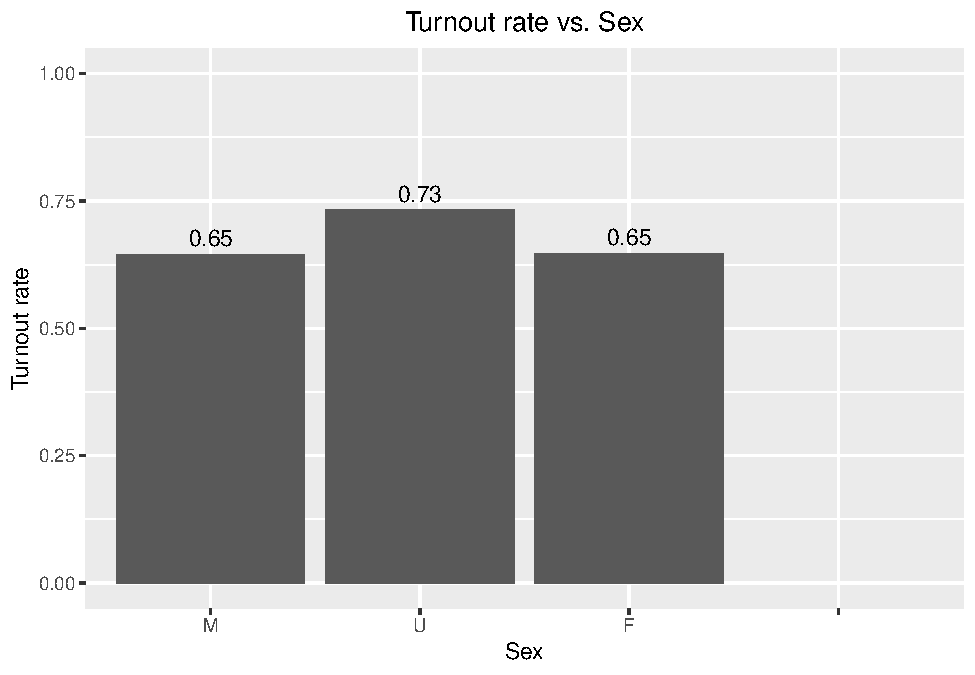
\includegraphics{CS2_files/figure-latex/unnamed-chunk-12-1.pdf}

\hypertarget{age}{%
\subsubsection{age}\label{age}}

\begin{Shaded}
\begin{Highlighting}[]
\NormalTok{data }\SpecialCharTok{\%\textgreater{}\%}
  \FunctionTok{group\_by}\NormalTok{(age) }\SpecialCharTok{\%\textgreater{}\%}
  \FunctionTok{summarise}\NormalTok{(}\AttributeTok{total\_reg =} \FunctionTok{sum}\NormalTok{(total\_reg),}
            \AttributeTok{total\_vot =} \FunctionTok{sum}\NormalTok{(total\_vot), }\AttributeTok{.groups =} \StringTok{"drop"}\NormalTok{) }\SpecialCharTok{\%\textgreater{}\%}
  \FunctionTok{mutate}\NormalTok{(}\AttributeTok{turnout\_rate =}\NormalTok{ total\_vot }\SpecialCharTok{/}\NormalTok{ total\_reg) }\SpecialCharTok{\%\textgreater{}\%}
  \FunctionTok{select}\NormalTok{(}\AttributeTok{group =}\NormalTok{ age, turnout\_rate) }\SpecialCharTok{\%\textgreater{}\%}
  \FunctionTok{ggplot}\NormalTok{( }\FunctionTok{aes}\NormalTok{(}\AttributeTok{x =}\NormalTok{ group, }\AttributeTok{y =}\NormalTok{ turnout\_rate)) }\SpecialCharTok{+}
  \FunctionTok{geom\_bar}\NormalTok{(}\AttributeTok{stat =} \StringTok{"identity"}\NormalTok{) }\SpecialCharTok{+}
  \FunctionTok{ylim}\NormalTok{(}\DecValTok{0}\NormalTok{,}\DecValTok{1}\NormalTok{) }\SpecialCharTok{+}
  \FunctionTok{xlab}\NormalTok{(}\StringTok{"Age"}\NormalTok{) }\SpecialCharTok{+} \FunctionTok{ylab}\NormalTok{(}\StringTok{"Turnout rate"}\NormalTok{) }\SpecialCharTok{+}
  \FunctionTok{geom\_text}\NormalTok{(}\FunctionTok{aes}\NormalTok{(}\AttributeTok{label=}\FunctionTok{format}\NormalTok{(turnout\_rate, }\AttributeTok{digits =} \DecValTok{2}\NormalTok{)), }\AttributeTok{vjust =} \SpecialCharTok{{-}}\FloatTok{0.5}\NormalTok{) }\SpecialCharTok{+}
  \FunctionTok{ggtitle}\NormalTok{(}\StringTok{"Turnout rate vs. Age"}\NormalTok{) }\SpecialCharTok{+}
    \FunctionTok{theme}\NormalTok{(}\AttributeTok{plot.title =} \FunctionTok{element\_text}\NormalTok{(}\AttributeTok{hjust =} \FloatTok{0.5}\NormalTok{))}
\end{Highlighting}
\end{Shaded}

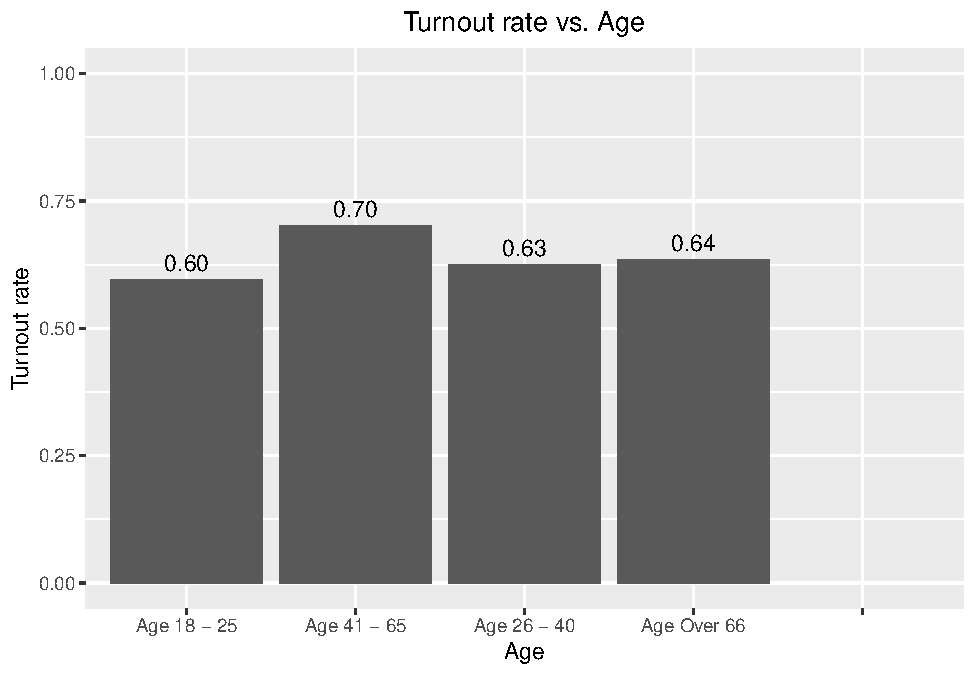
\includegraphics{CS2_files/figure-latex/unnamed-chunk-13-1.pdf}

\hypertarget{sex-party}{%
\subsubsection{sex \& party}\label{sex-party}}

\begin{Shaded}
\begin{Highlighting}[]
\NormalTok{data }\SpecialCharTok{\%\textgreater{}\%}
  \FunctionTok{group\_by}\NormalTok{(sex\_code, party\_cd) }\SpecialCharTok{\%\textgreater{}\%}
  \FunctionTok{summarise}\NormalTok{(}\AttributeTok{total\_reg =} \FunctionTok{sum}\NormalTok{(total\_reg),}
            \AttributeTok{total\_vot =} \FunctionTok{sum}\NormalTok{(total\_vot), }\AttributeTok{.groups =} \StringTok{"drop"}\NormalTok{) }\SpecialCharTok{\%\textgreater{}\%}
  \FunctionTok{mutate}\NormalTok{(}\AttributeTok{turnout\_rate =}\NormalTok{ total\_vot }\SpecialCharTok{/}\NormalTok{ total\_reg,}
         \AttributeTok{group =} \FunctionTok{paste0}\NormalTok{(sex\_code, }\StringTok{" with "}\NormalTok{, party\_cd)) }\SpecialCharTok{\%\textgreater{}\%}
  \FunctionTok{select}\NormalTok{(}\AttributeTok{group =}\NormalTok{ group, turnout\_rate, sex\_code, party\_cd) }\SpecialCharTok{\%\textgreater{}\%}
  \FunctionTok{ggplot}\NormalTok{( }\FunctionTok{aes}\NormalTok{(}\AttributeTok{x =}\NormalTok{ group, }\AttributeTok{y =}\NormalTok{ turnout\_rate, }\AttributeTok{fill =}\NormalTok{ sex\_code)) }\SpecialCharTok{+}
  \FunctionTok{geom\_bar}\NormalTok{(}\AttributeTok{stat =} \StringTok{"identity"}\NormalTok{) }\SpecialCharTok{+}
  \FunctionTok{ylim}\NormalTok{(}\DecValTok{0}\NormalTok{,}\DecValTok{1}\NormalTok{) }\SpecialCharTok{+}
  \FunctionTok{xlab}\NormalTok{(}\StringTok{"Sex * Party"}\NormalTok{) }\SpecialCharTok{+} \FunctionTok{ylab}\NormalTok{(}\StringTok{"Turnout rate"}\NormalTok{) }\SpecialCharTok{+}
  \FunctionTok{geom\_text}\NormalTok{(}\FunctionTok{aes}\NormalTok{(}\AttributeTok{label=}\FunctionTok{format}\NormalTok{(turnout\_rate, }\AttributeTok{digits =} \DecValTok{2}\NormalTok{)), }\AttributeTok{hjust =} \SpecialCharTok{{-}}\FloatTok{0.3}\NormalTok{) }\SpecialCharTok{+}
  \FunctionTok{coord\_flip}\NormalTok{() }\SpecialCharTok{+}
  \FunctionTok{ggtitle}\NormalTok{(}\StringTok{"Turnout rate vs. Sex*Party"}\NormalTok{) }\SpecialCharTok{+}
    \FunctionTok{theme}\NormalTok{(}\AttributeTok{plot.title =} \FunctionTok{element\_text}\NormalTok{(}\AttributeTok{hjust =} \FloatTok{0.5}\NormalTok{))}
\end{Highlighting}
\end{Shaded}

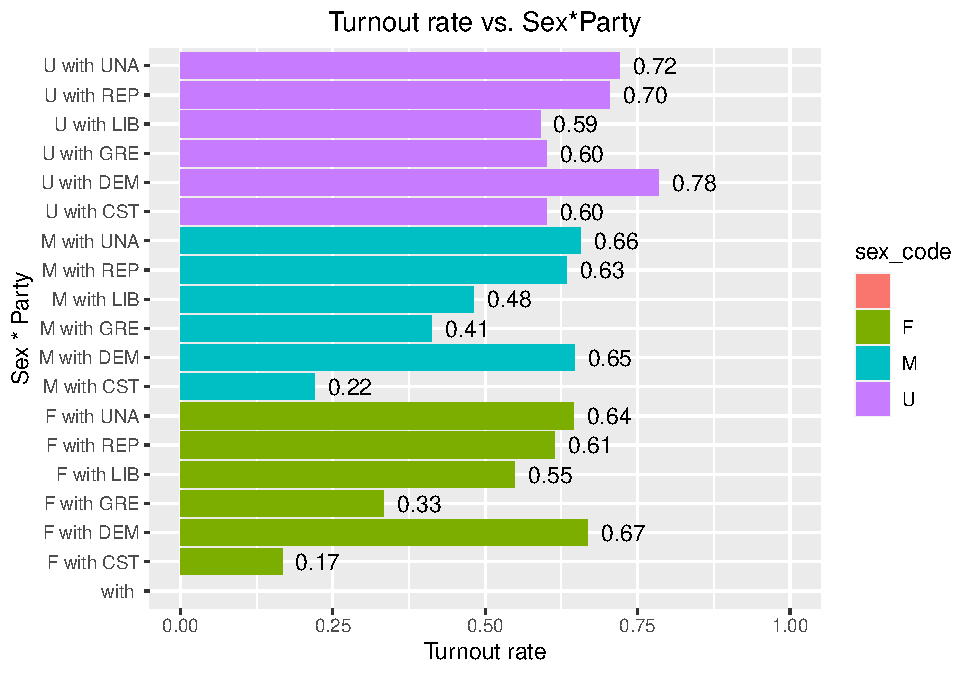
\includegraphics{CS2_files/figure-latex/unnamed-chunk-14-1.pdf}

\hypertarget{age-party}{%
\subsubsection{age \& party}\label{age-party}}

\begin{Shaded}
\begin{Highlighting}[]
\NormalTok{data }\SpecialCharTok{\%\textgreater{}\%}
  \FunctionTok{group\_by}\NormalTok{(age, party\_cd) }\SpecialCharTok{\%\textgreater{}\%}
  \FunctionTok{summarise}\NormalTok{(}\AttributeTok{total\_reg =} \FunctionTok{sum}\NormalTok{(total\_reg),}
            \AttributeTok{total\_vot =} \FunctionTok{sum}\NormalTok{(total\_vot), }\AttributeTok{.groups =} \StringTok{"drop"}\NormalTok{) }\SpecialCharTok{\%\textgreater{}\%}
  \FunctionTok{mutate}\NormalTok{(}\AttributeTok{turnout\_rate =}\NormalTok{ total\_vot }\SpecialCharTok{/}\NormalTok{ total\_reg,}
         \AttributeTok{group =} \FunctionTok{paste0}\NormalTok{(age, }\StringTok{" with "}\NormalTok{, party\_cd)) }\SpecialCharTok{\%\textgreater{}\%}
  \FunctionTok{select}\NormalTok{(}\AttributeTok{group =}\NormalTok{ group, turnout\_rate, age, party\_cd) }\SpecialCharTok{\%\textgreater{}\%}
  \FunctionTok{ggplot}\NormalTok{( }\FunctionTok{aes}\NormalTok{(}\AttributeTok{x =}\NormalTok{ group, }\AttributeTok{y =}\NormalTok{ turnout\_rate, }\AttributeTok{fill =}\NormalTok{ age)) }\SpecialCharTok{+}
  \FunctionTok{geom\_bar}\NormalTok{(}\AttributeTok{stat =} \StringTok{"identity"}\NormalTok{) }\SpecialCharTok{+}
  \FunctionTok{ylim}\NormalTok{(}\DecValTok{0}\NormalTok{,}\DecValTok{1}\NormalTok{) }\SpecialCharTok{+}
  \FunctionTok{xlab}\NormalTok{(}\StringTok{"Age * Party"}\NormalTok{) }\SpecialCharTok{+} \FunctionTok{ylab}\NormalTok{(}\StringTok{"Turnout rate"}\NormalTok{) }\SpecialCharTok{+}
  \FunctionTok{geom\_text}\NormalTok{(}\FunctionTok{aes}\NormalTok{(}\AttributeTok{label=}\FunctionTok{format}\NormalTok{(turnout\_rate, }\AttributeTok{digits =} \DecValTok{2}\NormalTok{)), }\AttributeTok{hjust =} \SpecialCharTok{{-}}\FloatTok{0.3}\NormalTok{) }\SpecialCharTok{+}
  \FunctionTok{coord\_flip}\NormalTok{() }\SpecialCharTok{+}
  \FunctionTok{ggtitle}\NormalTok{(}\StringTok{"Turnout rate vs. Age*Party"}\NormalTok{) }\SpecialCharTok{+}
    \FunctionTok{theme}\NormalTok{(}\AttributeTok{plot.title =} \FunctionTok{element\_text}\NormalTok{(}\AttributeTok{hjust =} \FloatTok{0.5}\NormalTok{))}
\end{Highlighting}
\end{Shaded}

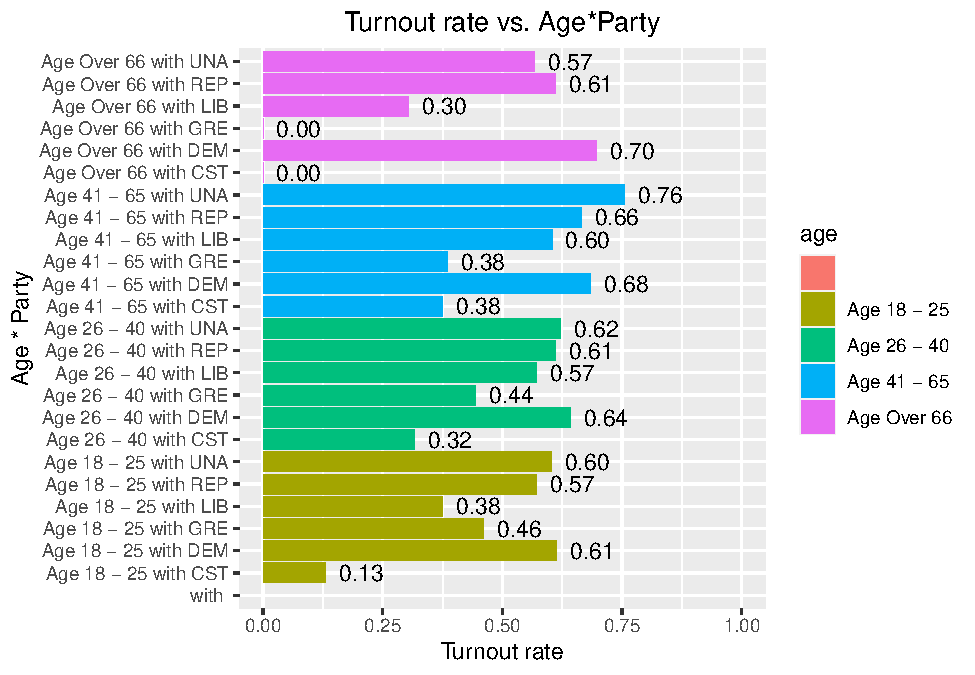
\includegraphics{CS2_files/figure-latex/unnamed-chunk-15-1.pdf}

\hypertarget{age-race}{%
\subsubsection{age \& race}\label{age-race}}

\begin{Shaded}
\begin{Highlighting}[]
\NormalTok{data }\SpecialCharTok{\%\textgreater{}\%}
  \FunctionTok{group\_by}\NormalTok{(age, race\_code) }\SpecialCharTok{\%\textgreater{}\%}
  \FunctionTok{summarise}\NormalTok{(}\AttributeTok{total\_reg =} \FunctionTok{sum}\NormalTok{(total\_reg),}
            \AttributeTok{total\_vot =} \FunctionTok{sum}\NormalTok{(total\_vot), }\AttributeTok{.groups =} \StringTok{"drop"}\NormalTok{) }\SpecialCharTok{\%\textgreater{}\%}
  \FunctionTok{mutate}\NormalTok{(}\AttributeTok{turnout\_rate =}\NormalTok{ total\_vot }\SpecialCharTok{/}\NormalTok{ total\_reg,}
         \AttributeTok{group =} \FunctionTok{paste0}\NormalTok{(age, }\StringTok{" with "}\NormalTok{, race\_code)) }\SpecialCharTok{\%\textgreater{}\%}
  \FunctionTok{select}\NormalTok{(}\AttributeTok{group =}\NormalTok{ group, turnout\_rate, age, race\_code) }\SpecialCharTok{\%\textgreater{}\%}
  \FunctionTok{ggplot}\NormalTok{( }\FunctionTok{aes}\NormalTok{(}\AttributeTok{x =}\NormalTok{ group, }\AttributeTok{y =}\NormalTok{ turnout\_rate, }\AttributeTok{fill =}\NormalTok{ age)) }\SpecialCharTok{+}
  \FunctionTok{geom\_bar}\NormalTok{(}\AttributeTok{stat =} \StringTok{"identity"}\NormalTok{) }\SpecialCharTok{+}
  \FunctionTok{ylim}\NormalTok{(}\DecValTok{0}\NormalTok{,}\DecValTok{1}\NormalTok{) }\SpecialCharTok{+}
  \FunctionTok{xlab}\NormalTok{(}\StringTok{"Age * Race"}\NormalTok{) }\SpecialCharTok{+} \FunctionTok{ylab}\NormalTok{(}\StringTok{"Turnout rate"}\NormalTok{) }\SpecialCharTok{+}
  \FunctionTok{geom\_text}\NormalTok{(}\FunctionTok{aes}\NormalTok{(}\AttributeTok{label=}\FunctionTok{format}\NormalTok{(turnout\_rate, }\AttributeTok{digits =} \DecValTok{2}\NormalTok{)), }\AttributeTok{hjust =} \SpecialCharTok{{-}}\FloatTok{0.3}\NormalTok{) }\SpecialCharTok{+}
  \FunctionTok{coord\_flip}\NormalTok{() }\SpecialCharTok{+}
  \FunctionTok{ggtitle}\NormalTok{(}\StringTok{"Turnout rate vs. Age*Race"}\NormalTok{) }\SpecialCharTok{+}
    \FunctionTok{theme}\NormalTok{(}\AttributeTok{plot.title =} \FunctionTok{element\_text}\NormalTok{(}\AttributeTok{hjust =} \FloatTok{0.5}\NormalTok{))}
\end{Highlighting}
\end{Shaded}

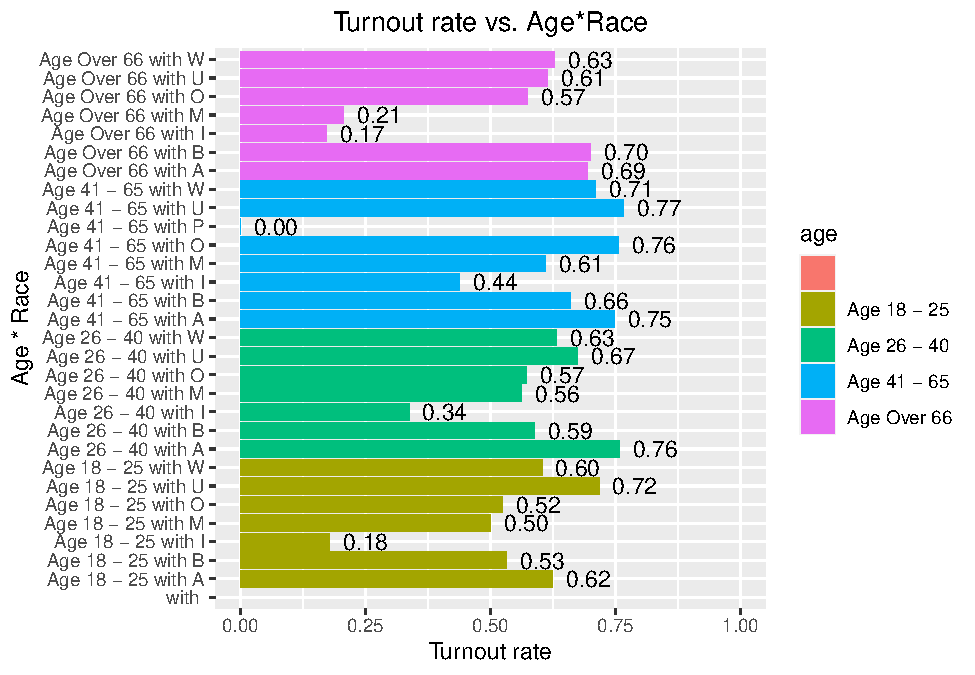
\includegraphics{CS2_files/figure-latex/unnamed-chunk-16-1.pdf}

\hypertarget{model}{%
\section{Model}\label{model}}

In order to answer the questions of interest, we require the following
features in our model:

\begin{enumerate}
\def\labelenumi{\arabic{enumi}.}
\tightlist
\item
  Fixed effects for various demographic subgroups (race, ethnicity, age,
  sex)
\item
  Random effects for county
\item
  Sex-Party interaction
\item
  Age-Party interaction
\end{enumerate}

\begin{Shaded}
\begin{Highlighting}[]
\NormalTok{mod1 }\OtherTok{\textless{}{-}} \FunctionTok{glmer}\NormalTok{(}\FunctionTok{cbind}\NormalTok{(total\_vot, total\_reg }\SpecialCharTok{{-}}\NormalTok{ total\_vot) }\SpecialCharTok{\textasciitilde{}}
                      \DecValTok{1} \SpecialCharTok{+}\NormalTok{ (}\DecValTok{1}\SpecialCharTok{|}\NormalTok{county\_desc),}
                    \AttributeTok{data =}\NormalTok{ data, }\AttributeTok{family =}\NormalTok{ binomial,}
              \AttributeTok{control=}\FunctionTok{glmerControl}\NormalTok{(}\AttributeTok{optimizer =} \StringTok{"bobyqa"}\NormalTok{))}
\end{Highlighting}
\end{Shaded}

\begin{Shaded}
\begin{Highlighting}[]
\FunctionTok{as.data.frame}\NormalTok{(}\FunctionTok{summary}\NormalTok{(mod1)}\SpecialCharTok{$}\NormalTok{coefficients) }\SpecialCharTok{\%\textgreater{}\%}
  \FunctionTok{mutate}\NormalTok{(}\StringTok{\textasciigrave{}}\AttributeTok{95\% CI}\StringTok{\textasciigrave{}} \OtherTok{=} \FunctionTok{paste0}\NormalTok{(}
    \StringTok{\textquotesingle{}[\textquotesingle{}}\NormalTok{, }
    \FunctionTok{round}\NormalTok{(Estimate }\SpecialCharTok{{-}} \FloatTok{1.96} \SpecialCharTok{*} \StringTok{\textasciigrave{}}\AttributeTok{Std. Error}\StringTok{\textasciigrave{}}\NormalTok{, }\DecValTok{3}\NormalTok{), }\StringTok{\textquotesingle{}, \textquotesingle{}}\NormalTok{, }
    \FunctionTok{round}\NormalTok{(Estimate }\SpecialCharTok{+} \FloatTok{1.96} \SpecialCharTok{*} \StringTok{\textasciigrave{}}\AttributeTok{Std. Error}\StringTok{\textasciigrave{}}\NormalTok{, }\DecValTok{3}\NormalTok{), }\StringTok{\textquotesingle{}]\textquotesingle{}}\NormalTok{ )}
\NormalTok{  ) }\SpecialCharTok{\%\textgreater{}\%}
  \FunctionTok{select}\NormalTok{(Estimate, }\StringTok{\textasciigrave{}}\AttributeTok{95\% CI}\StringTok{\textasciigrave{}}\NormalTok{) }\SpecialCharTok{\%\textgreater{}\%}
  \FunctionTok{kable}\NormalTok{(}\AttributeTok{digits=}\DecValTok{3}\NormalTok{) }\SpecialCharTok{\%\textgreater{}\%}
  \FunctionTok{kable\_styling}\NormalTok{(}\AttributeTok{full\_width=}\ConstantTok{FALSE}\NormalTok{) }\SpecialCharTok{\%\textgreater{}\%}
  \FunctionTok{kable\_classic}\NormalTok{()}
\end{Highlighting}
\end{Shaded}

\begin{table}
\centering
\begin{tabular}{l|r|l}
\hline
  & Estimate & 95\% CI\\
\hline
(Intercept) & -0.372 & [-0.659, -0.086]\\
\hline
\end{tabular}
\end{table}

\begin{Shaded}
\begin{Highlighting}[]
 \CommentTok{\# glmer(cbind(cbind(total\_vot, total\_reg {-} total\_vot) \textasciitilde{}}
 \CommentTok{\#                  party\_cd + race\_code + ethnic\_code + sex\_code + age +}
 \CommentTok{\#                  sex\_code:party\_cd + age:party\_cd + age:race\_code + (1|county\_desc),}
 \CommentTok{\#                data = data, family = binomial)}
\end{Highlighting}
\end{Shaded}


\end{document}
